\documentclass[conference]{IEEEtran}
\IEEEoverridecommandlockouts
\usepackage[T1]{fontenc}
\usepackage{graphicx,amsmath,amssymb,booktabs,cite,url}
\usepackage{eso-pic}
\AddToShipoutPictureBG{%
\put(\LenToUnit{\paperwidth-0.5cm},\LenToUnit{\paperheight-1.2cm}){%
\makebox(0,0)[r]{\footnotesize 24BCE1993-Divyanth Dayasankar.P,\ 24BCE5108-Rohit Michael Raj}}}
% Generated from saved model_metrics, benchmark_results, secretbook_latency_results, and dataset manifest.
\newcommand{\FinalN}{76,323}
\newcommand{\TrainN}{56,422}
\newcommand{\ValN}{10,022}
\newcommand{\TestN}{9,879}
\newcommand{\TestAccuracy}{98.17}
\newcommand{\CsicAccuracy}{95.72}
\newcommand{\ValAccuracy}{98.28}
\newcommand{\FalsePositives}{41}
\newcommand{\FalseNegatives}{140}
\newcommand{\TrueNegatives}{4,441}
\newcommand{\TruePositives}{5,257}
\newcommand{\XaiCoverage}{100.00}
\newcommand{\ForwardMean}{0.270}
\newcommand{\XaiMean}{0.653}
\newcommand{\HttpMean}{3.435}
\newcommand{\VocabN}{116}
\newcommand{\ParameterN}{30,625}
\newcommand{\SelectedEpoch}{11}
\newcommand{\EpochsRun}{12}
\newcommand{\TrainingSeconds}{247.5}
\newcommand{\Threshold}{0.45}
\newcommand{\CiLow}{97.88}
\newcommand{\CiHigh}{98.41}
\newcommand{\RocAuc}{0.9976}
\newcommand{\AveragePrecision}{0.9982}
\newcommand{\Fpr}{0.91}
\newcommand{\Fnr}{2.59}
\newcommand{\LoadingMs}{4.145}
\newcommand{\FirstForward}{1.509}
\newcommand{\Throughput}{3,445}
\newcommand{\XaiPninetyfive}{0.814}
\newcommand{\TopDrop}{11.098}
\newcommand{\RandomDrop}{1.925}
\newcommand{\TopWins}{100.00}
\newcommand{\MarkerMatch}{90.00}
\newcommand{\SmokeCorrect}{20}
\newcommand{\SmokeTN}{10}
\newcommand{\SmokeFP}{0}
\newcommand{\SmokeFN}{0}
\newcommand{\SmokeTP}{10}
\newcommand{\SplitRows}{Train & 30,090 & 26,332 & 56,422\\
Validation & 4,736 & 5,286 & 10,022\\
Test & 4,482 & 5,397 & 9,879\\
\midrule
Total & 39,308 & 37,015 & 76,323\\}
\newcommand{\ClassRows}{Normal & 0.9694 & 0.9909 & 0.9800 & 4,482\\
Attack/anomaly & 0.9923 & 0.9741 & 0.9831 & 5,397\\}
\newcommand{\SourceRows}{SQLI & 4,468 & 99.80 & 0.9979\\
XSS & 1,649 & 99.33 & 0.9920\\
CSIC & 3,762 & 95.72 & 0.9518\\}
\newcommand{\LatencyRows}{CNN forward & 0.270 & 0.214 & 0.441\\
Detector incl. encoding & 0.290 & 0.231 & 0.483\\
Attribution only & 0.653 & 0.623 & 0.814\\
WAF + trivial view & 0.603 & 0.681 & 1.010\\
Trivial response only & 0.008 & 0.008 & 0.010\\
Loopback HTTP & 3.435 & 1.477 & 20.214\\}
\newcommand{\SecretBookRequests}{700}
\newcommand{\SecretBookPageMin}{3.006}
\newcommand{\SecretBookPageMax}{5.284}
\newcommand{\SecretBookBlockMin}{3.722}
\newcommand{\SecretBookBlockMax}{4.689}
\newcommand{\SecretBookForwardMin}{0.307}
\newcommand{\SecretBookForwardMax}{0.318}
\newcommand{\SecretBookAttributionMin}{0.741}
\newcommand{\SecretBookAttributionMax}{0.753}
\newcommand{\SecretBookRows}{Home (scored) & 200 & 0.664 & 3.006 & 14.481\\
Login & 200 & 0.901 & 3.314 & 18.942\\
Signup & 200 & 0.831 & 5.284 & 25.110\\
Feed redirect & 302 & 0.629 & 3.456 & 16.247\\
XSS block & 403 & 1.361 & 3.722 & 16.935\\
SQLi block & 403 & 1.346 & 4.689 & 24.225\\
Home (bypass) & 200 & 0.306 & 4.029 & 23.749\\}

\title{Lightweight Explainable Runtime Detection of SQL Injection, XSS, and Anomalous HTTP Requests in Django}
\author{\IEEEauthorblockN{Divyanth Dayasankar.P, Rohit Michael Raj}
\IEEEauthorblockA{\textit{Department of Computer Science}\\\textit{VIT Chennai}\\Chennai, India}}
\begin{document}
\maketitle
\begin{abstract}
A request detector must distinguish attacks from legitimate application inputs, account for related examples across dataset partitions, and expose the scope of its timing measurements. We implement a character-level convolutional neural network (CNN) as early Django middleware and evaluate a combined SQLi, XSS, and CSIC HTTP corpus. Shared canonicalization, conflicting-label quarantine, and group-based partitioning produce \FinalN{} final examples: \TrainN{} training, \ValN{} validation, and \TestN{} test requests after training-only deployment augmentation. A training-derived vocabulary and overlapping 256-character windows avoid vocabulary leakage and the earlier last-100-character blind spot. Validation-based model selection yields \TestAccuracy{}\% accuracy on the reused fixed test, with \FalsePositives{} false positives and \FalseNegatives{} false negatives; CSIC subset accuracy is \CsicAccuracy{}\%. Logit-gradient-times-embedding attribution explains blocks without differentiating a saturated sigmoid, returning spans for all 100 sampled correctly blocked test attacks. Across \SecretBookRequests{} sequential anonymous HTTP requests to the actual SecretBook application, endpoint mean round-trip latency is \SecretBookPageMin{}--\SecretBookPageMax{} ms for scored home, login and signup pages, and \SecretBookBlockMin{}--\SecretBookBlockMax{} ms for SQLi/XSS blocks with HTML explanations. Separate warm CPU benchmarks measure \ForwardMean{} ms forward and \XaiMean{} ms attribution latency. These local prototype results do not establish concurrent production performance or independent unseen-family generalization.
\end{abstract}
\begin{IEEEkeywords}
web application firewall, character CNN, SQL injection, XSS, HTTP anomaly detection, explainable AI, Django
\end{IEEEkeywords}

\section{Introduction}
SQL injection and cross-site scripting exploit how an application interprets untrusted inputs. Parameterized queries, output escaping, access control, and framework protections remain necessary when an additional request detector is deployed. A learned detector can provide a supplementary decision before application processing, but offline accuracy alone does not establish that it will accept normal traffic or identify the region responsible for a block.

This work studies these engineering and evaluation questions together in a Django research prototype. Inputs are the request path and query string plus supported textual body content. Outputs are a binary attack/anomaly score and, for a block, local character attribution. Adding CSIC broadens the positive class: its anomalies are not exclusively SQLi or XSS and include invalid application inputs~\cite{csic}. The model does not identify a verified exploit type.

An audit of the preceding prototype found stale dataset paths, identical encoded inputs shared across train/test partitions, vocabulary construction before splitting, and a last-100-character input restriction. Earlier latency claims confused direct inference with middleware execution, and saturated predictions could produce no explanatory spans. This revision addresses these defects and documents remaining limits.

The contributions are: (1) one versioned combined dataset with provenance, exclusion accounting, and fixed partitions; (2) shared training/runtime scoring with overlapping-window coverage within an explicit limit; (3) bounded early Django enforcement with logit-based attribution; and (4) separate classification, explanation-sensitivity, inference, middleware, and loopback HTTP measurements. The contribution is an auditable integrated prototype rather than a new attribution algorithm or a claim to outperform all WAFs.

\section{Related Work}
Character-level CNNs classify text without a word tokenizer or pretrained language model~\cite{charcnn}. Request punctuation, markup, and encoded sequences make this approach relevant. Our compact network uses three convolutional layers and max/average pooling rather than the original large text-classification architecture.

Tadhani et al.~\cite{tadhani} combine decoding and standardization with CNN--LSTM detection. They report 99.84\% accuracy on SQL--XSS payloads, 99.77\% on HTTP CSIC 2010, and 99.23\% on a custom testbed. These are results under their own procedures, not baselines rerun in this project. Bak{\i}r's UniEmbed~\cite{uniembed} fuses Word2Vec, FastText, and Universal Sentence Encoder into 712 features and compares classifiers, reporting 99.82\% XSS MLP accuracy. We do not assign unmeasured latency to either approach or claim a controlled accuracy ranking.

Ancona et al.~\cite{ancona} analyze gradient attribution and its sensitivity. We use gradient-times-embedding with the pre-sigmoid attack logit as its target. Saliency is not causal proof or verified exploit evidence; prior sanity-check work motivates evaluating explanation behavior~\cite{sanity}. Our masking comparison is a limited sensitivity diagnostic, not a replacement for expert annotation or randomization studies.

\section{Dataset and Evaluation Protocol}
\subsection{Input Scope and Provenance}
The supplied files contain 30,919 SQLiV3 rows, 13,686 XSS rows, and 61,065 CSIC rows. CSIC has 36,000 normal and 25,065 anomalous labels. We use its URL and content fields, removing host/scheme and the trailing HTTP version. The textual class column, classification field, cookies, and other headers are excluded from model inputs. This avoids class-bearing metadata and matches middleware visibility. Source hashes identify the exact local CSVs; we do not assume they are identical to their original published exports.

Both benign and attack SQLi/XSS payloads use the same \texttt{/search?q=} wrapper. Output rows retain a sample hash, source and row number, combined duplicate provenance, group identifier, encoded-input hash, augmentation designation, and split. One final CSV and three split CSVs accompany a JSON manifest. Labels are not flipped to obtain a desired accuracy.

\subsection{Shared Normalization and Cleaning}
Dataset construction and runtime import the same normalization function: Unicode NFKC, at most two HTML-unescape/URL-decode passes, whitespace folding, trimming, and lowercasing. NUL characters become a literal escape marker. Normalized text exceeding 4,096 characters is outside the inspection scope.

From 105,670 raw rows, 310 invalid/missing SQLi rows are removed. Two examples exceed the normalized length limit. All 6,404 rows involved in conflicting normalized-input labels are quarantined, rather than selecting a preferred label. Another 32,541 duplicate normalized rows are collapsed, retaining provenance. This leaves 66,413 source-derived inputs. Excluding conflicts is material: identical detector-visible representations can have different labels when relevant context is omitted, and the resulting task is cleaner than raw traffic.

\subsection{Group Splits and Deployment Adaptation}
Grouping keys strip the common search wrapper and replace long hexadecimal strings and digit runs. Twenty stratified group folds use seed 42; 14 are training, three validation, and three test, approximating 70/15/15 while preserving groups. Source-derived membership is 46,512 training, 10,022 validation, and 9,879 test requests. Vocabulary uses training characters only, with separate padding and unknown indices.

A first model using only these inputs reached 98.63\% test accuracy but blocked eight of ten benign development smoke requests. Training-only adaptation added 6,910 benign deployment examples and 3,000 wrappers derived exclusively from 1,500 training attacks. Added examples cover navigation, forms, JSON-like bodies, educational SQL text, and ambiguous benign keywords. Attack variants retain their parent group. Validation and test sample identities were preserved.

This development sequence is disclosed because the test had been inspected before adaptation. Final checkpoint and threshold selection still use validation only, but the test is a reused holdout, not a wholly untouched external evaluation. The smoke suite also overlaps deployment-development patterns and is not independent evidence.

\begin{table}[t]
\centering
\caption{Final partitions after training-only augmentation}
\label{tab:splits}
\begin{tabular}{lrrr}
\toprule
Partition & Normal & Attack/anomaly & Total\\
\midrule
\SplitRows
\bottomrule
\end{tabular}
\end{table}

The audit finds no shared group identifiers or identical complete encoded requests across splits. The \VocabN{}-character training vocabulary is frozen before test encoding; unknown characters map to 1 and padding to 0. Grouping controls the specified transformations, not every semantic attack family. Common fragments and application structures may remain shared.

\section{Detection and Explainability}
\subsection{Windowed Character CNN}
Requests are covered by 256-character windows at stride 192, adding an aligned final window to cover the suffix. Short inputs are left-padded; no admitted normalized character is dropped. Each window uses a 32-dimensional embedding, Conv1D layers with 64, 64, and 32 channels (kernel three, padding one, ReLU), and adaptive max/average pooling. Their 64-dimensional concatenation enters a 64-to-32 layer, ReLU, dropout 0.30, and a scalar logit layer. The model contains \ParameterN{} parameters.

For windows $w_1,\ldots,w_m$, document scoring is
\begin{equation}
z(x)=\max_{1\le j\le m}f_\theta(w_j),\qquad p(x)=\sigma(z(x)).
\end{equation}
Training and runtime use the same aggregation. One high-scoring window can block a request. This avoids suffix-only inspection, but maximum aggregation can amplify false positives in longer requests. Full character coverage is not guaranteed exploit detection.

\begin{figure*}[t]
\centering
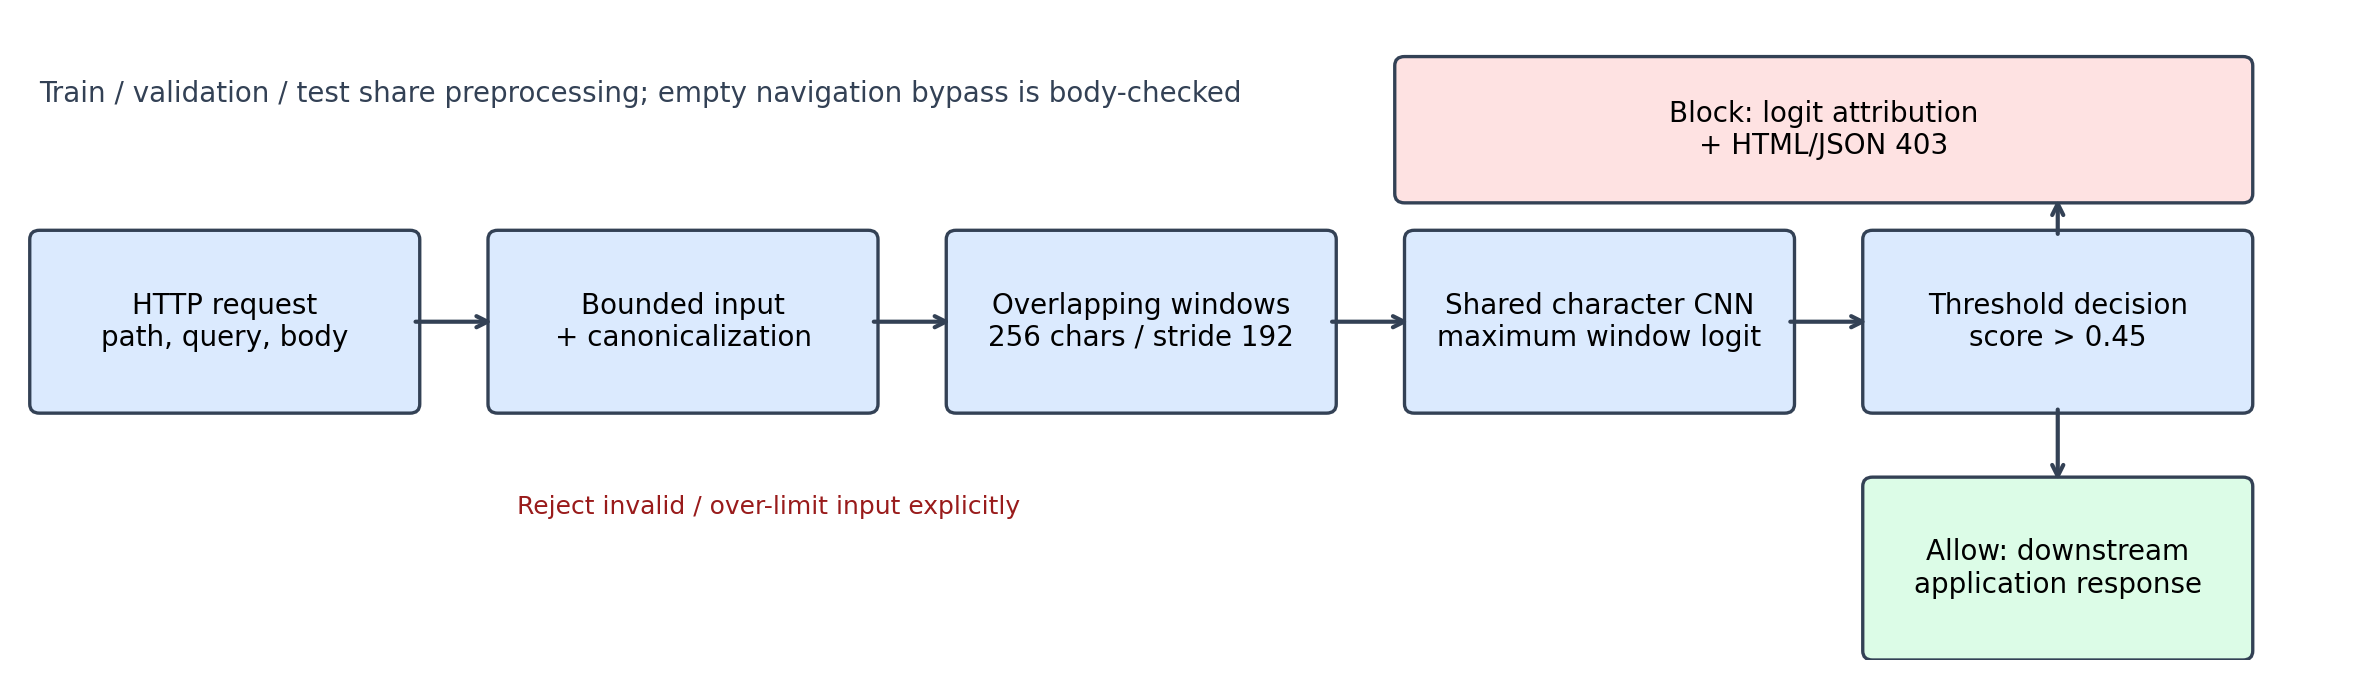
\includegraphics[width=.94\textwidth]{architecture.png}
\caption{Shared preprocessing and CNN code. Out-of-scope requests are rejected explicitly; admitted requests are scored across all windows. Attribution targets the winning window's logit.}
\label{fig:architecture}
\end{figure*}

\subsection{Training and Selection}
Training uses seed 42, deterministic CPU operations, two PyTorch threads, batch size 128, and Adam~\cite{adam} with learning rate $10^{-3}$ and weight decay $10^{-4}$. With training class ratio $a=N_0/N_1$, weighted binary cross-entropy is
\begin{equation}
\mathcal L=-\frac{1}{N}\sum_{i=1}^N
\left[a\,y_i\log p_i+(1-y_i)\log(1-p_i)\right].
\end{equation}
Implementation uses \texttt{BCEWithLogitsLoss}. ReduceLROnPlateau monitors validation loss with factor 0.5 and patience one. Training allows 12 epochs and early stopping after three non-improving epochs. Epoch \SelectedEpoch{} was selected from \EpochsRun{} completed epochs by minimum validation weighted loss; training took \TrainingSeconds{} seconds.

Thresholds from 0.10 to 0.90 in steps of 0.01 are evaluated on validation macro-F1, breaking ties toward 0.5. The selected threshold is \Threshold{}, with strict blocking at $p(x)>\Threshold{}$. Validation accuracy is \ValAccuracy{}\%. Neither label corruption nor accuracy-targeted checkpoint selection is used.

\begin{figure}[t]
\centering
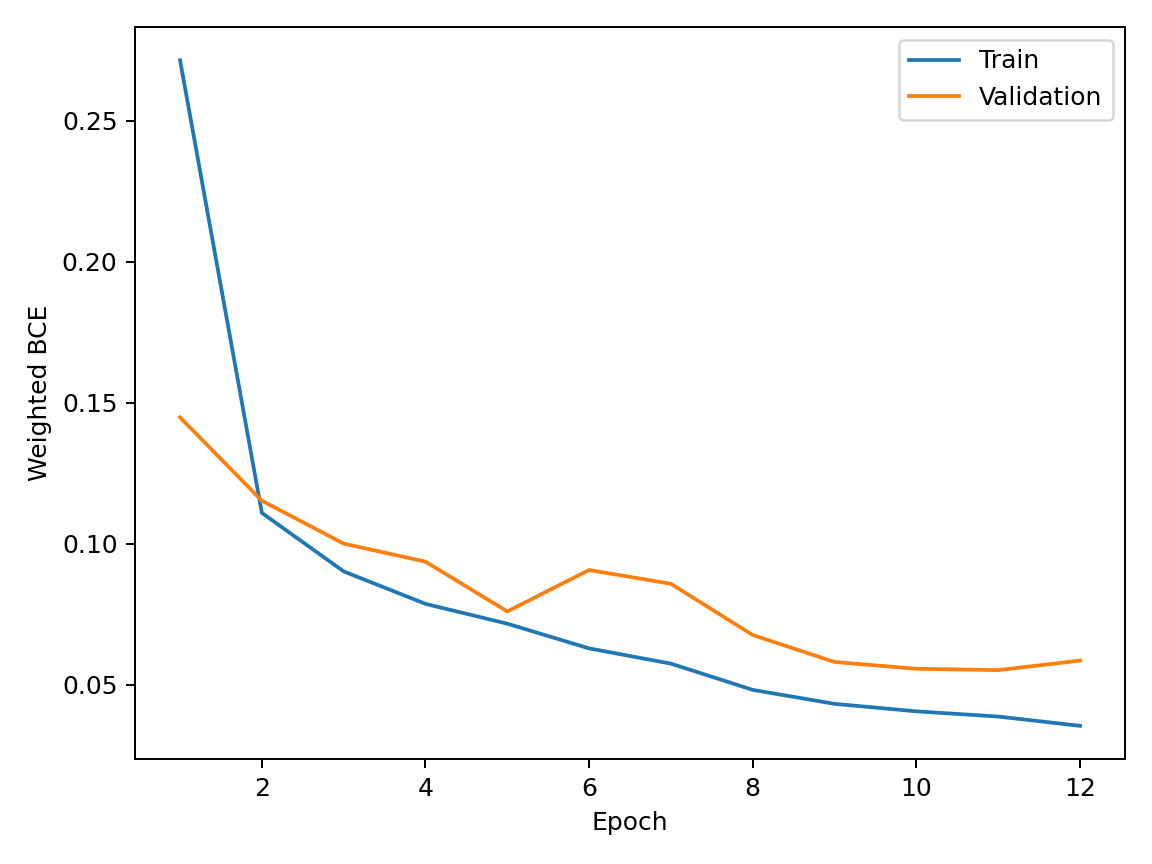
\includegraphics[width=.47\textwidth]{training_curve.png}
\caption{Training and validation weighted loss. Selection uses validation loss, not test accuracy.}
\end{figure}

\subsection{Logit-Based Local Attribution}
For embedding $E_{i,d}$ of character $i$, the winning-window attribution is
\begin{equation}
s_i=\sum_d\left|E_{i,d}\frac{\partial f_\theta(w)}{\partial E_{i,d}}\right|.
\end{equation}
The target is the unsquashed logit. Differentiating a saturated sigmoid can otherwise erase gradients despite confident blocking. A regression test verifies attribution when the reported probability rounds to one. The implementation uses \texttt{autograd.grad} on detached embeddings, avoiding mutation of shared parameter gradients.

Attributions are normalized by their maximum. Values at least the greater of the 75th percentile and 0.20 are selected, consecutive characters are joined, and ten context characters are added on each side. Up to three spans are returned, skipping candidates contained in already selected spans. Offsets refer to the complete normalized request, not raw HTTP bytes. If all saliency is zero, the response reports that attribution is unavailable; explanatory evidence is never invented.

\subsection{Django Integration and Correctness}
AttackDetectionMiddleware follows SecurityMiddleware and precedes session, authentication, view, and database work. A bounded read admits at most 16,384 body bytes and preserves admitted bytes for downstream parsing. Invalid framing yields 400; oversized bodies or normalized text 413; excessive raw URLs 414; unsupported nonempty body types 415. Supported bodies include JSON, URL-encoded forms, text, XML, and bounded multipart text fields. Uploaded file contents are not scored.

Known navigation routes bypass inference only for GET/HEAD requests without queries and with a body proven empty by the bounded read. Other admitted requests are scored. Blocks return HTML or JSON HTTP 403 with score, random reference, and available influential spans. Logs contain references, methods, decisions and timings, not request paths or payloads. Scores are not calibrated exploit probabilities.

Application corrections include ownership-filtered edit/delete lookup, deliberate responses for invalid forms, preservation of creation timestamps, newest-first feeds, and authenticated CSRF-protected POST post deletion. Account deletion uses GET confirmation and CSRF-protected POST mutation. Host defaults are local. These are prototype correctness improvements, not comprehensive production hardening.

\section{Experimental Results}
\subsection{Classification}
Final test accuracy is \TestAccuracy{}\%, with a sample-level Wilson 95\% interval of \CiLow{}--\CiHigh{}\%, ROC-AUC \RocAuc{}, and average precision \AveragePrecision{}. The interval assumes independent requests; remaining correlations can make it overconfident. These are pooled binary-label metrics, not attack-category identification.

\begin{table}[t]
\centering
\caption{Final fixed-test classification}
\begin{tabular}{lrrrr}
\toprule
Class & Precision & Recall & F1 & Support\\
\midrule
\ClassRows
\bottomrule
\end{tabular}
\end{table}

\begin{figure}[t]
\centering
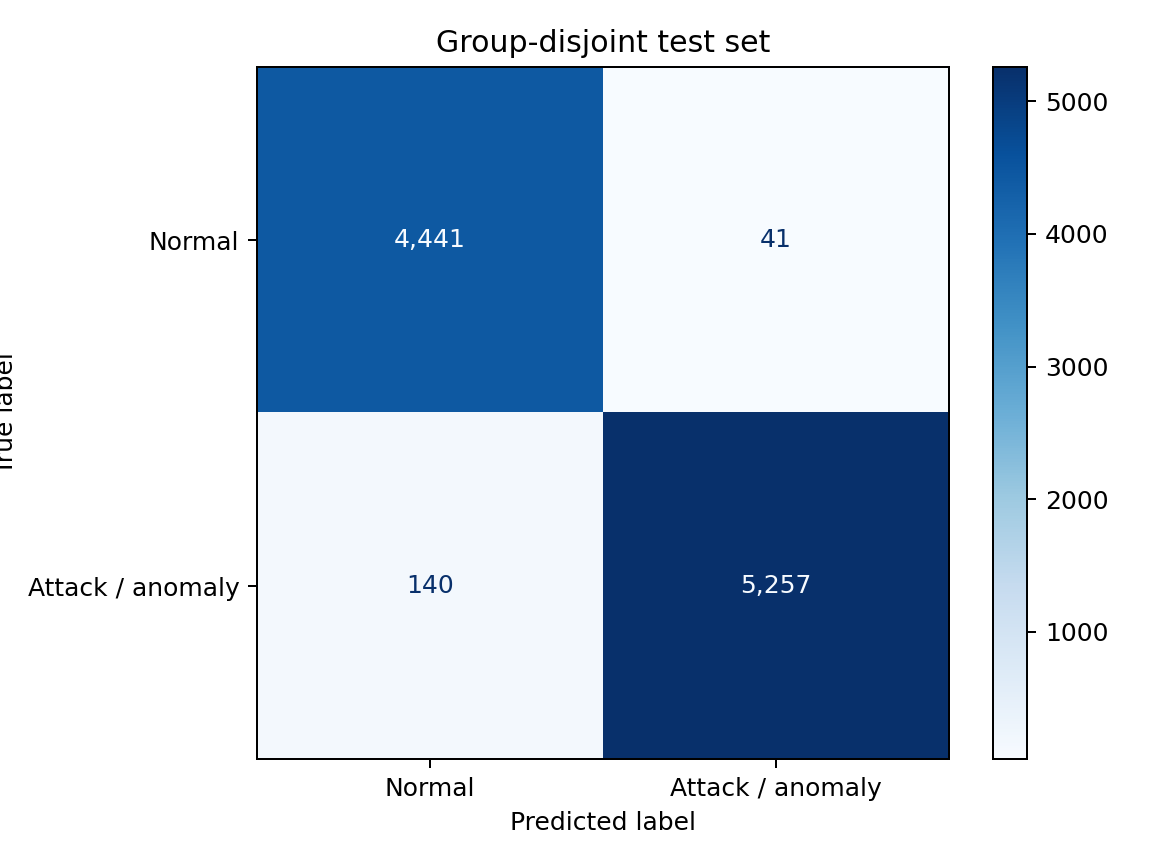
\includegraphics[width=.45\textwidth]{confusion_matrix.png}
\caption{Final test confusion matrix; both error types remain nonzero.}
\end{figure}

There are \TrueNegatives{} true negatives, \FalsePositives{} false positives, \FalseNegatives{} false negatives, and \TruePositives{} true positives. False-positive and false-negative rates are \Fpr{}\% and \Fnr{}\%, respectively. Source-specific results expose differences hidden by pooled accuracy.

\begin{table}[t]
\centering
\caption{Test results by retained source representative}
\begin{tabular}{lrrr}
\toprule
Source & Samples & Accuracy (\%) & Macro-F1\\
\midrule
\SourceRows
\bottomrule
\end{tabular}
\end{table}

\subsection{Latency and Scope}
Benchmarks use Windows on an AMD64 CPU, Python 3.14.3, PyTorch 2.10.0+cpu, NumPy 2.3.5, and two threads. Training uses Python 3.10.8 and PyTorch 2.7.0 on CPU. Model loading takes \LoadingMs{} ms and the first forward call \FirstForward{} ms; neither is included in warm statistics.

The warm benchmark cycles through 512 seeded test inputs for 1,000 calls. Forward time includes all windows and maximum-score selection but excludes encoding. Detector-total time adds encoding and result construction; inputs are already normalized. The middleware benchmark uses the 20 development requests, disables navigation bypass to force inference, enables explanations and JSON blocks, and calls a trivial view on allowed traffic. RequestFactory construction is outside its timer. The baseline measures construction of the trivial response.

A separate loopback benchmark sends actual TCP HTTP requests to a single-thread WSGI server containing the real WAF and a trivial view, with 20 warmups and 100 measurements. It includes connection, parsing, enforcement, response generation and transport, but excludes TLS, sessions, authentication, database work and concurrent load. It is not a complete SecretBook page benchmark. No percentage overhead is inferred from an assumed typical request time.

\begin{table}[t]
\centering
\caption{Measured latency in milliseconds, by scope}
\begin{tabular}{lrrr}
\toprule
Scope & Mean & Median & p95\\
\midrule
\LatencyRows
\bottomrule
\end{tabular}
\end{table}
Sequential detector throughput including encoding, but excluding normalization and explanations, is \Throughput{} requests/s. HTTP tail latency is reported even when considerably higher than its median; forward latency must not substitute for round-trip latency.

\subsection{Full SecretBook HTTP Measurements}
An additional experiment runs the actual SecretBook WSGI application with its complete configured middleware, URL resolution and templates over loopback TCP. Seven request cases receive ten warmups and 100 measured anonymous GET requests each (\SecretBookRequests{} measurements). Model inference remains enabled on the scored routes, while the query-free home navigation case exercises the documented bypass. Both attack cases return HTTP 403 with nonempty HTML explanatory regions. Table~\ref{tab:secretbook} separates instrumented Django application time from client-observed HTTP round-trip time.

Each measurement opens a new HTTP connection and reads the complete response. The Django timer covers WSGI application execution, response iteration and closure; the client timer additionally includes connection setup and transport. Endpoint mean forward times within these live requests range from \SecretBookForwardMin{} to \SecretBookForwardMax{} ms. Mean attribution times are \SecretBookAttributionMin{}--\SecretBookAttributionMax{} ms across the two blocked cases and are already included in their Django and HTTP totals.

\begin{table}[t]
\centering
\caption{Actual SecretBook latency (ms); mean unless marked p95}
\label{tab:secretbook}
\begin{tabular}{lrrrr}
\toprule
Endpoint & Status & Django & HTTP & HTTP p95\\
\midrule
\SecretBookRows
\bottomrule
\end{tabular}
\end{table}

Database instrumentation records zero queries for these anonymous requests: the feed endpoint redirects to login rather than rendering authenticated posts. These measurements include real application HTML rendering and configured request handling, but exclude logged-in database workloads, browser subresources, TLS, redirect following and concurrency. The WAF plus trivial-view benchmark above remains a distinct experiment. Its numbers must not be presented as full SecretBook page latency.

The reported ranges summarize endpoint means, not individual-request bounds. HTTP p95 values are substantially larger than Django application means. The bypass and scored cases have different inputs and are measured sequentially, so subtracting their round-trip means would not isolate WAF overhead. These observations establish measured local response times, not a guaranteed real-time deadline.

\subsection{Explanation Evaluation}
The first 100 correctly blocked attacks in seeded test order have returned-span coverage of \XaiCoverage{}\%, mean attribution latency \XaiMean{} ms, and p95 \XaiPninetyfive{} ms. This measures availability among true positives, not explanations for missed attacks.

For a matched-size sensitivity comparison, the top 10\% of winning-window characters by attribution are masked to padding. Ten random masks of equal size form the comparison per request. Mean window-logit decrease is \TopDrop{} for top-attribution masking and \RandomDrop{} for random masking; the former is greater in \TopWins{}\% of examples. These changes concern the winning-window logit, not necessarily the final document decision, because another window can become maximal.

\begin{figure}[t]
\centering
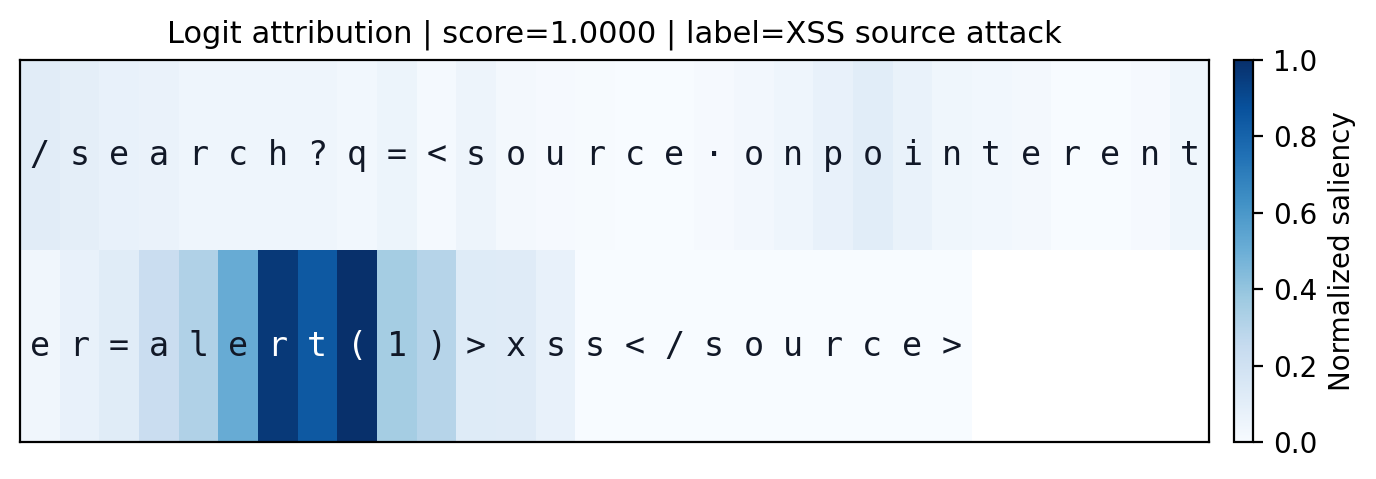
\includegraphics[width=.47\textwidth]{explanation_example.png}
\caption{Character attribution for a deterministically selected correctly blocked XSS test example. Color denotes sensitivity, not exploit severity.}
\end{figure}
The development marker heuristic finds an SQL/HTML marker in \MarkerMatch{}\% of correctly blocked smoke attacks. Substring matching is weak evidence: short markers can match accidentally, and useful spans may omit them. Masking is more informative but can create out-of-distribution inputs. No human validation, causal study, or full randomization-based saliency assessment was performed.

\subsection{Runtime Regression}
The development suite contains ten benign and ten attack inputs. The final detector makes \SmokeCorrect{}/20 correct decisions: \SmokeTN{} TN, \SmokeFP{} FP, \SmokeFN{} FN, and \SmokeTP{} TP. Its purpose is regression diagnosis; some patterns are represented in deployment training. Tests additionally exercise the saved model through real JSON-body middleware, scored benign forwarding, body-bearing GET/HEAD requests on bypass paths, multipart and URL-encoded bodies, bounded reads, invalid framing, full window coverage, saturation-resistant attribution, ownership, and deletion semantics.

\section{Discussion and Limitations}
\textbf{Generalization.} Group separation removes exact request overlap and specified numeric/hex variants, not complete attack techniques or applications. CSIC includes invalid but not necessarily malicious traffic; headers and files remain outside the representation. The model is a binary attack/anomaly detector for the stated inputs, not a definitive exploit verifier.

\textbf{Exclusions and reuse.} Uniform conflict quarantine makes labeling well-defined for the selected representation but can simplify the task. The fixed test was inspected after the first model and reused following smoke-driven deployment adaptation. Neither that reuse nor development smoke performance establishes external validity.

\textbf{Operational limits.} Oversized or unsupported requests are explicitly rejected. This can reject legitimate uploads and large API bodies, so limits must fit the application. A tightly scoped navigation bypass remains a separate runtime path. Window maxima avoid silent suffix truncation but can increase false positives as the number of windows grows.

\textbf{Attribution and cost.} Logit attribution addresses sigmoid saturation, yet nonzero saliency is not guaranteed for every future input. Sensitivity can highlight punctuation or benign context and does not prove causation. Timing depends on hardware, request length, threads, explanation frequency and transport. Sequential throughput cannot establish concurrent production performance.

\textbf{Comparisons.} The cited CNN--LSTM and UniEmbed results use different datasets and protocols. We make no ranking against them or ModSecurity. Controlled future comparisons should rerun baselines on identical partitions and hardware, use source-held-out data, and include false positives and explanation costs.

\section{Conclusion}
The revised prototype combines SQLi, XSS and CSIC data with traceable partitions, training-only vocabulary construction, and deployment augmentation. Shared overlapping-window scoring, bounded Django inspection, and logit-gradient explanations correct defects in the earlier implementation. The selected model achieves \TestAccuracy{}\% accuracy on the reused fixed test and \CsicAccuracy{}\% on its CSIC subset. Integration is exercised by \SecretBookRequests{} real HTTP requests through SecretBook: endpoint mean round-trip latency is \SecretBookPageMin{}--\SecretBookPageMax{} ms for the three scored pages and \SecretBookBlockMin{}--\SecretBookBlockMax{} ms for attack blocks including HTML explanations. Independent warm measurements report \ForwardMean{} ms forward and \XaiMean{} ms attribution latency. The results support feasibility for the measured local anonymous workload; authenticated database traffic and concurrent deployment remain unevaluated.

Future work should collect independent application traffic, group by broader attack families, study calibrated thresholds at realistic class prevalence, assess explanation robustness with expert and randomization controls, and benchmark concurrent full-application traffic. Conventional secure coding and framework protections remain essential.

\section*{Acknowledgment}
The authors thank the dataset contributors and VIT Chennai. Exact local exports and hashes are recorded in the manifest; original SQLi/XSS export provenance could not be conclusively established from filenames alone.

\begin{thebibliography}{9}
\bibitem{csic}
C. Torrano Gim\'enez, A. P\'erez Villegas, and G. \'Alvarez Mara\~n\'on, \emph{HTTP Dataset CSIC 2010}, CSIC, 2010. Archived dataset description. [Online]. Available: \url{https://petescully.co.uk/wp-content/uploads/2018/04/http_dataset_csic_2010.pdf}
\bibitem{charcnn}
X. Zhang, J. Zhao, and Y. LeCun, \emph{Character-level convolutional networks for text classification}, in Advances in Neural Information Processing Systems, vol. 28, 2015. [Online]. Available: \url{https://arxiv.org/abs/1509.01626}
\bibitem{tadhani}
J. R. Tadhani, V. Vekariya, V. Sorathiya, S. Alshathri, and W. El-Shafai, \emph{Securing web applications against XSS and SQLi attacks using a novel deep learning approach}, Scientific Reports, vol. 14, art. 1803, 2024, doi: 10.1038/s41598-023-48845-4.
\bibitem{uniembed}
R. Bak{\i}r, \emph{UniEmbed: A novel approach to detect XSS and SQL injection attacks leveraging multiple feature fusion with machine learning techniques}, Arabian Journal for Science and Engineering, 2025, doi: 10.1007/s13369-024-09916-4.
\bibitem{ancona}
M. Ancona, E. Ceolini, C. \"Oztireli, and M. Gross, \emph{Towards better understanding of gradient-based attribution methods for deep neural networks}, in ICLR, 2018. [Online]. Available: \url{https://arxiv.org/abs/1711.06104}
\bibitem{sanity}
J. Adebayo et al., \emph{Sanity checks for saliency maps}, in Advances in Neural Information Processing Systems, 2018. [Online]. Available: \url{https://arxiv.org/abs/1810.03292}
\bibitem{adam}
D. P. Kingma and J. Ba, \emph{Adam: A method for stochastic optimization}, in ICLR, 2015. [Online]. Available: \url{https://arxiv.org/abs/1412.6980}
\end{thebibliography}
\end{document}
